The use of representation models for retrieval begins with a document space $d$ and a query space $q$ where, each of which is generated by some model $m$. Models do not need to share the same initialization, shape, or size, but their representation vectors must share size without some projection. These two models learn a notion of relevance by training to minimize the distance of positive query-document pairs as shown in equation \ref{eq:dis} where $\textbf{x}$ is a query vector and $\textbf{y}$ is a document vector, and $\cdot$ denotes the dot product of the vectors.\\
\begin{equation}
L = 1 - \frac{\textbf{x} \cdot \textbf{y}}{|\textbf{x}||\textbf{y}|}
 \label{eq:dis}
\end{equation}
The query and document encoder models are commonly initialized with a pre-trained language model such as BERT. Then, using pairs of labels for positive relevance scores for queries and documents, the models are trained to minimize the distance between queries and their relevant documents \cite{Karpukhin2020DensePR} \\
\begin{figure}[!htb]
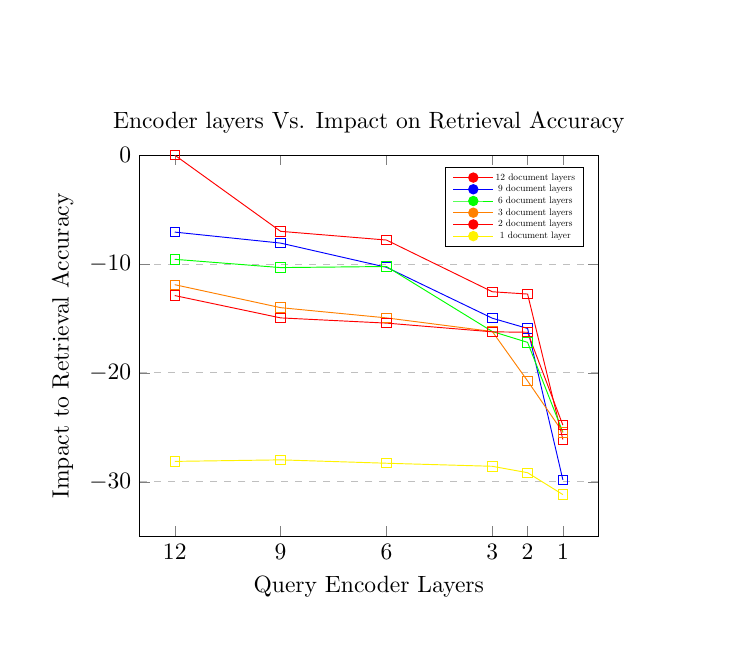
\begin{tikzpicture}
\scalebox{0.85}{
\begin{axis}[
    title={Encoder layers Vs. Impact on Retrieval Accuracy   },
    xlabel={Query Encoder Layers},
    ylabel={Impact to Retrieval Accuracy},
    xmin=0, xmax=13,
    x dir=reverse,
    ymin=-35 , ymax=0,
    xtick={1,2,3,6,9,12},
    ytick={0, -10,-20,-30},
    legend pos=north east,
    ymajorgrids=true,
    grid style=dashed,
    legend style={nodes={scale=0.4, transform shape}}, 
    legend image post style={mark=*}
]
\addplot[
    color=red,
    mark=square,
    ]
    coordinates {
    (12, 0) (9, -7.00) (6,-7.8) (3,-12.55) (2, -12.76) (1, -26.12)
    };

\addplot[
    color=blue,
    mark=square,
    ]
    coordinates {
    (12, -7.07) (9, -8.08) (6,-10.3) (3,-14.98) (2, -15.92) (1, -29.83)

    };

\addplot[
    color=green,
    mark=square,
    ]
    coordinates {
    (12, -9.57) (9, -10.33) (6,-10.23) (3,-16.2) (2, -17.2) (1, -25.46)
    };


\addplot[
    color=orange,
    mark=square,
    ]
    coordinates {
    (12, -11.9) (9, -14.01) (6,-14.95) (3,-16.2) (2, -20.74) (1, -25.46)
    };
\addplot[
    color=red,
    mark=square,
    ]
    coordinates {
    (12, -12.90) (9, -14.95) (6,-15.43) (3,-16.23) (2, -16.27) (1, -24.8)
    };

\addplot[
    color=yellow,
    mark=square,
    ]
    coordinates {
    (12, -28.13) (9, -27.99) (6,-28.3) (3,-28.58) (2, -29.17) (1, -31.18)
    };
\legend{12 document layers, 9 document layers, 6 document layers, 3 document layers, 2 document layers, 1 document layer }
 \end{axis}}

\end{tikzpicture}
    \centering
    \caption{Measuring the impact on recall at 20 on the NQ retrieval dataset by varying the number of transformer layers for the query encoder and document encoder \label{fig:asm-1}}
\end{figure}
While it is common practice to initialize the query encoder and document encoder with identical language models, this ignores the cost asymmetry of the usage patterns. The document encoder is usually only used once during a large-scale batch generation of the index. Index generation happens in a latency-insensitive environment and can easily leverage many GPUs and large batch sizes to improve efficiency.\\
The query encoder runs every time a user issues a query, which can be irregular and sporadically. The query encoder responds to each user query independently. Thus, query encoders often use a batch size of 1 and commonly leverage small inference-optimized hardware like the T4 GPU or small CPUs. \\
Since the document encoder does not run very often, any improvement in latency produces a single fixed gain utterly dependent on the corpus size and index refresh cycle. The query encoder's user-facing nature means latency improvements occur whenever a user queries. 
\subsection{Role of model symmetry with Bi-encoders}
The variation in latency sensitivity between the query and document encoder leads to the question: Is there some form of asymmetry between the query encoder and the document encoder that can be exploited? Do the two encoders need to be compressed symmetrically? \\
To answer this question, we explore the impact on the performance of pruning the query and document encoders on the NQ passage retrieval dataset \cite{Kwiatkowski2019NaturalQA}. Using a BERT-base uncased model with 12 transformer encoder layers, we generate structurally pruned models with 9,6,3,2 and 1 layers. We also further pre-train the three and six-layer models using knowledge distillation, represented as $6_{KD}$ and $3_{KD}$, from a 12-layer model on the Wikipedia-book corpus similar to distilBERT \cite{sanh2019distilbert}. \\
Then, using each of these seven models, we train dense retrieval models on the NQ passage retrieval dataset with variations of query and document models resulting in 72 variants. With each of these models, we generate a full index and evaluate retrieval performance on the development portion of the dataset. We do not tune any parameters to avoid overfitting and to explore asymmetry without overoptimizing. Each model's retrieval accuracy is evaluated with retrieval sets of depth 20, 100, and 200. We compare the impact of varying the encoders to the uncompressed baseline and a distilBERT model (denoted by $6_{db}$. \\
\begin{table}[!htb]
    \centering
    \caption{Impact of Structural pruning before fine-tuning on Retrieval Accuracy on NQ passage retrieval dataset}
    \scalebox{0.6}{\begin{tabular}{|l|l|l|l|l|l|l|}
    \hline        Layers $enc$ & Top 20 & Impact & Top 100 & Impact & Top 200 & Impact \\ \hline
        12 & 79.86\% & 0.00\% & 85.84\% & 0.00\% & 88.42\% & 0.00\% \\ \hline
        $6_{db}$ & 73.88\% & -7.49\% & 84.74\% & -1.29\% & 87.26\% & -1.31\% \\ \hline
        9 & 73.41\% & -8.08\% & 83.68\% & -2.51\% & 86.51\% & -2.16\% \\ \hline
        $6_{KD}$ & 75.04\% & -8.08\% & 85.15\% & -0.80\% & 87.45\% & -1.10\% \\ \hline
        6 & 71.69\% & -8.08\% & 83.30\% & -2.96\% & 86.04\% & -2.69\% \\ \hline
        $3_{KD}$ & 73.32\% & -8.08\% & 83.43\% & -2.80\% & 86.20\% & -2.51\% \\ \hline
        3 & 66.93\% & -16.20\% & 80.61\% & -6.09\% & 84.49\% & -4.45\% \\ \hline
        2 & 66.87\% & -16.27\% & 80.42\% & -6.32\% & 83.85\% & -5.17\% \\ \hline
        1 & 54.96\% & -31.18\% & 71.88\% & -16.26\% & 76.73\% & -13.22\% \\ \hline
    \end{tabular}}
    \label{tab:sym-nq}
\end{table}
Looking at the impact of symmetric compression as shown in table \ref{tab:sym-nq}, we see that the impact of compression is more pronounced with a small recall set as retrieval accuracy impact at 20 is ~3x that of at 200. We also observe major accuracy gains by fine-tuning the pruned model with a 4\% gap for the 6-layer model and a 6\% gap for the 3-layer model for recall at 20. \\
We find that the document encoder drives retrieval accuracy by looking at the results of asymmetrical training in table \ref{tab:asym-nq}. As shown in figure \ref{fig:asm-1}, retrieval accuracy is driven by the document encoder following prior work showing performance out of domain is dependent on the document encoder \cite{Li2021EncoderAO}. \\
The size of the Document encoder sets the upper bound on a model's performance as a model with 12 layers in the query encoder, and 9 in the document encoder performs worse than one with the numbers flipped. The dominance of the document encoder is a logical outcome, as the latent space for queries is simpler than the latent space for documents. As a result, system performance is governed by how well the document encoder can generate representations. \\
Similar results can be seen with the introduction of fine-tuned three and 6-layer models as shown in \ref{tab:asym-nq-kd}. Unsurprisingly, KD-optimized language models outperform non-distilled models, and any asymmetrical variant that leverages a distilled model outperforms the un-distilled variant. Without further optimization, a model with a distilled 3-layer query encoder and a 12-layer document encoder will outperform a model with symmetrical 6-layer models despite being 2x faster. \\
\begin{table}[!htb]
    \centering
    \caption{Impact of Structural pruning before fine-tuning on Retrieval Accuracy on NQ passage retrieval dataset}
    \scalebox{0.5}{
    \begin{tabular}{|l|l|l|l|l|l|l|l|}
    \hline
        $layers_{q}$ & $layers_{d}$ & Top 20 & Impact & Top 100 & Impact & Top 200 & Impact \\ \hline
        12 & 12 & 79.86\% & 0.00\% & 85.84\% & 0.00\% & 88.42\% & 0.00\% \\ \hline
        \midrule

        9 & 12 & 74.27\% & -7.00\% & 84.40\% & -1.67\% & 86.95\% & -1.66\% \\ \hline
        6 & 12 & 73.63\% & -7.80\% & 84.27\% & -1.83\% & 86.79\% & -1.85\% \\ \hline
        3 & 12 & 69.83\% & -12.55\% & 82.58\% & -3.80\% & 85.35\% & -3.48\% \\ \hline
        2 & 12 & 69.67\% & -12.76\% & 82.19\% & -4.25\% & 84.68\% & -4.23\% \\ \hline
        1 & 12 & 59.00\% & -26.12\% & 75.37\% & -12.19\% & 81.00\% & -8.39\% \\ \hline
        \midrule
        12 & 9 & 74.21\% & -7.07\% & 84.40\% & -1.67\% & 87.06\% & -1.53\% \\ \hline
        9 & 9 & 73.41\% & -8.08\% & 83.68\% & -2.51\% & 86.51\% & -2.16\% \\ \hline
        6 & 9 & 71.63\% & -10.30\% & 83.05\% & -3.25\% & 85.98\% & -2.76\% \\ \hline
        3 & 9 & 67.89\% & -14.98\% & 80.94\% & -5.71\% & 84.79\% & -4.10\% \\ \hline
        2 & 9 & 67.15\% & -15.92\% & 80.53\% & -6.19\% & 83.66\% & -5.39\% \\ \hline
        1 & 9 & 56.04\% & -29.83\% & 73.35\% & -14.55\% & 78.12\% & -11.65\% \\ \hline
        \midrule
        12 & 6 & 72.22\% & -9.57\% & 83.41\% & -2.83\% & 85.84\% & -2.91\% \\ \hline
        9 & 6 & 71.61\% & -10.33\% & 83.30\% & -2.96\% & 85.93\% & -2.82\% \\ \hline
        6 & 6 & 71.69\% & -10.23\% & 83.30\% & -2.96\% & 86.04\% & -2.69\% \\ \hline
        3 & 6 & 66.93\% & -16.20\% & 80.28\% & -6.48\% & 83.96\% & -5.04\% \\ \hline
        2 & 6 & 66.12\% & -17.20\% & 80.33\% & -6.42\% & 83.49\% & -5.58\% \\ \hline
        1 & 6 & 59.53\% & -25.46\% & 75.37\% & -12.19\% & 79.83\% & -9.71\% \\ \hline
        \midrule
        12 & 3 & 70.36\% & -11.90\% & 81.72\% & -4.80\% & 84.60\% & -4.32\% \\ \hline
        9 & 3 & 68.67\% & -14.01\% & 80.47\% & -6.25\% & 84.46\% & -4.48\% \\ \hline
        6 & 3 & 67.92\% & -14.95\% & 80.06\% & -6.74\% & 83.85\% & -5.17\% \\ \hline
        3 & 3 & 66.93\% & -16.20\% & 80.61\% & -6.09\% & 84.49\% & -4.45\% \\ \hline
        2 & 3 & 63.30\% & -20.74\% & 78.37\% & -8.71\% & 83.02\% & -6.11\% \\ \hline
        1 & 3 & 59.53\% & -25.46\% & 75.68\% & -11.84\% & 80.08\% & -9.43\% \\ \hline
        \midrule
        12 & 2 & 69.56\% & -12.90\% & 81.33\% & -5.25\% & 84.49\% & -4.45\% \\ \hline
        9 & 2 & 67.92\% & -14.95\% & 80.75\% & -5.93\% & 84.32\% & -4.64\% \\ \hline
        6 & 2 & 67.53\% & -15.43\% & 80.33\% & -6.42\% & 83.82\% & -5.20\% \\ \hline
        3 & 2 & 66.90\% & -16.23\% & 80.36\% & -6.38\% & 84.24\% & -4.73\% \\ \hline
        2 & 2 & 66.87\% & -16.27\% & 80.42\% & -6.32\% & 83.85\% & -5.17\% \\ \hline
        1 & 2 & 60.06\% & -24.80\% & 75.29\% & -12.29\% & 79.75\% & -9.80\% \\ \hline
        \midrule
        12 & 1 & 57.40\% & -28.13\% & 73.24\% & -14.68\% & 78.56\% & -11.15\% \\ \hline
        9 & 1 & 57.51\% & -27.99\% & 73.24\% & -14.68\% & 77.87\% & -11.94\% \\ \hline
        6 & 1 & 57.26\% & -28.30\% & 73.52\% & -14.35\% & 78.34\% & -11.40\% \\ \hline
        3 & 1 & 57.04\% & -28.58\% & 73.93\% & -13.87\% & 78.39\% & -11.34\% \\ \hline
        2 & 1 & 56.57\% & -29.17\% & 73.71\% & -14.13\% & 77.98\% & -11.81\% \\ \hline
        1 & 1 & 54.96\% & -31.18\% & 71.88\% & -16.26\% & 76.73\% & -13.22\% \\ \hline
    \end{tabular}}
    \label{tab:asym-nq}
\end{table}
\subsection{Inference Benchmarks}
To evaluate the impact of structural pruning, we benchmark inference speeds of query encoding while varying the number of transformer layers. We perform benchmarking using an Intel Xeon Gold 6238R Processor and a T4 Nvidia GPU. For each model, we evaluate the performance on encoding 6500 queries with a batch size of one and a max context length of 32. For CPU inference, we evaluate the performance of models using the ONNX library \footnote{https://onnx.ai/}, and for GPU inference, we evaluate native Pytorch inference. We repeat each run five times to ensure consistency and report the mean. Summary statistics can be found in \ref{tab:inference-summary} and full results, including percentile, standard deviation, and confidence intervals, can be found in the appendix \ref{sec:inference-benchmarks}.\\
\begin{table}[!ht]
    \centering
    \tiny
    \begin{tabular}{|l|l|l|l|l|l|}
    \hline
        layers & size & compressed size & method & QPS & Speedup \\ \hline
        12 & 418 & 387 & GPU & 105.852 & 1.00 \\ \hline
        9 & 337 & 212 & GPU & 139.494 & 1.32 \\ \hline
        6 & 256 & 236 & GPU & 172.338 & 1.63 \\ \hline
        3 & 175 & 161 & GPU & 299.45 & 2.83 \\ \hline
        2 & 148 & 136 & GPU & 441.422 & 4.17 \\ \hline
        1 & 121 & 111 & GPU & 660.64 & 6.24 \\ \hline
        12 & 418 & 387 & CPU & 47.278 & 1.00 \\ \hline
        9 & 337 & 212 & CPU & 63.24 & 1.34 \\ \hline
        6 & 256 & 236 & CPU & 90.386 & 1.91 \\ \hline
        3 & 175 & 161 & CPU & 166.012 & 3.51 \\ \hline
        2 & 148 & 136 & CPU & 229.666 & 4.86 \\ \hline
        1 & 121 & 111 & CPU & 378.534 & 8.01 \\ \hline
    \end{tabular}
    \caption{Variation in model throughput according to the serving method and the number of transformer layers. Structural pruning can lead to a 6 and 8-layer performance increase on GPU and CPU and pruning a model to 3 layers allows a CPU to offer better inference performance than the GPU.}
    \label{tab:inference-summary}
\end{table}